\documentclass{article}
\usepackage[utf8]{inputenc}
\usepackage{graphicx}
\usepackage{amsfonts}
\usepackage{amsmath}
\usepackage{biblatex}
\addbibresource{reference.bib}

\title{% 
Neural Ordinary Differential Equations \\
\large{Math 228A Final Project}}
\author{Longling Tian, Xuesi Ruan}
\date{November 2021}

\begin{document}

\maketitle

\begin{abstract}
    We introduce the basic concepts and functions of ODE solvers, neural networks, and neural ODEs. The most common and easiest algorithm is the Euler’s method, which leads to a residual neural network. In comparison, a neural ODE allows us to form an ODE neural network, which has less memory cost and increases accuracy. We go through the steps of backpropagation and the adjoint method in detail. We also discuss the application of neural ODE. By visualizing the loss and memory cost of both methods, we conclude that algorithms with ODE might not be the best approach in certain cases. When neural ODE fails, augmented neural ODE could be the improved solution to our problems.
\end{abstract}

\section{Introduction}

\subsection{Introduction to ODE solvers}

ODEs involve the evolution in time of one variable ($\mathbf{z}$), with the change in time being the derivative $\frac{d\mathbf{z}}{dt} = f(\mathbf{z}(t),t)$ {\cite{NODEvideo}}. Equivalently, $$\mathbf{z}(t_1) = \mathbf{z}(t_0) + \int_{\mathbf{z}(t_0)}^{\mathbf{z}(t_1)} f(\mathbf{z}(t), t)$$

There are plenty of ways to solve an ODE numerically with an initial condition. One of the most common algorithms is the Euler’s method, which approximates with small steps: $\mathbf{z}(t+\Delta h) = \mathbf{z}(t) + \Delta h f(\mathbf{z}, t)$.
However, this leads to large numerical errors and lots of memory. As a result, new adaptive ODE solvers have been developed over time to minimize the errors from previous steps. These different ODE solvers form the basic structures of different types of neural networks that we introduce in later sections.

\subsection{Introduction to neural network}
Neural networks play an important role in deep learning. A neural network consists of artificial nodes that imitate the operation of neurons in the human brain. It is composed of layers including one input layer, multiple hidden layers, and one output layer. The input layer receives numerical data values, which are assigned weights and biases by mathematical computations and passed onto the first hidden layer. The values run through the activation function which decides whether a neuron gets lit up, and the neurons that are on are passed down to the next hidden layer. The same procedure then gets iterated through the rest of the hidden layers on the remaining activated neurons. Lastly, the output layer returns the result, usually range from 0 to 1. This process is called forward propagation, however we use back propagation to achieve more accurate results because the weights are initialized to the inputs and adjusted every time for minimal error \cite{NduatiIntro}.

There are types of neural networks, with the most popular models being recurrent neural networks, convolutional networks, and neural differential equations. We are mainly going to focus on residual and ODE networks for the purpose of this paper. Unlike a purely residual neural network, incorporating ODE into a neural network has multiple advantages, namely memory efficiency, adaptive computation, and continuous time-series models \cite{chen2019neural}.

\subsection{Neural ODEs}
The focus of our paper is the black-box ODE solver. Instead of learning the specific transformation directly, the machine learning model learns the structure of transformations by solving the derivative of the original function as an ODE. 

We can produce an ODE neural network by backpropagate through the ODE solver for supervised learning. In Julia, we can implement the ODESolve() function to achieve this goal \cite{HoncharNODE}. Gradients can be computed using the adjoint method that solves a second and third augmented ODE backwards.

We will discuss the losses of neural ODE compared to common neural networks in detail later in the discussion section.

\subsection{Back-propagation and the adjoint method}

For a neural network model, the propagation steps are similar to the scheme of Euler's method. The whole transformation is composed of a sequence of hidden states $\mathbf{z}_i$, where $\mathbf{z}_{t+1} = \mathbf{z}_t + f(\mathbf{z}_t, \theta_t)$. Here $\theta$ represents model parameters which the neural network model optimizes.

When we add infinitely more layers and take infinitely smaller time steps, the hidden state dynamics could be specified by an ordinary differential equation: $\frac{d\mathbf{z}(t)}{dt} = f(\mathbf{z}(t), t, \theta)$. In this way, the output layer at given time $T$ becomes the solution of such ODE. The figure from Chen et.al contrasts discretized residual network and neural ODE network.

However, optimizing parameters is out of a black-box approach. We first define the loss function as the following:
$$L(\mathbf{z}({t_1}) = L(\mathbf{z}({t_0}) + \int_{t_0}^{t_1} f(\mathbf{z}(t), t, \theta){dt}) = L(\textup{ODESolve}(\mathbf{z}(t_0), f, {t_0}, {t_1}, \theta))$$
The first equality uses the definition of an ODE, and the second equality computes it using Julia function mentioned previously. To compute gradients, the most common way is the adjoint sensitivity method first emerged in 1962 by Pontryagin et.al. The adjoint is defined as $\mathbf{a}(t) = \frac{\partial{L}}{\partial\mathbf{z}}$, as the loss function with respect to the hidden state. By chain rule, we get $$\frac{\mathbf{a}(t)}{dt} = -\mathbf{a}(t) \frac{\partial{f}(\mathbf{z}(t), t, \theta)}{\partial\mathbf{z}(t)}$$ Therefore, $$\frac{\partial{L}}{\partial\mathbf{z}} = \mathbf{a}(t) =  \int_{t_1}^{t_0}\mathbf{a}(t) \frac{\partial{f}(\mathbf{z}(t), t, \theta)}{\partial\mathbf{z}(t)}$$ can be computed by a call of ODE solver according to the formula above. Note that this solver runs backwards, starting at $t_1$. This means the full trajectory is no longer required. One can recompute $\mathbf{h}(t)$ along the full trajectory only knowing the value of $\mathbf{h}(t_1)$ and the adjoint function $\mathbf{a}(t)$.

In a similar fashion, gradient with respect to model parameters $\theta$ can also be computed by a call to the ODE solver. $$\frac{\partial{L}}{\partial{\theta}} = -\int_{t_1}^{t_0}{\mathbf{a}(t) \frac{\partial{f}(\mathbf{z}(t), t, \theta)}{\partial\theta}}$$

Chen et.al presented a innovative approach to concatenate the original state, adjoint, and the partial derivative $\frac{\partial{L}}{\partial{\theta}}$ into a single vector called the augmented adjoint: $$\mathbf{a}_{aug} = \begin{bmatrix}
\mathbf{a} \\
\mathbf{a}_\theta \\
\mathbf{a}_t
\end{bmatrix},
\frac{d\mathbf{a}_{aug}}{dt} = -\mathbf{a}\begin{bmatrix}
\partial f / \partial \mathbf{z} \\
\partial f / \partial \theta \\
\partial f / \partial t
\end{bmatrix}
$$

In this way, the entire back-propagation algorithm can be evaluated by a single call to the ODE solver. $\mathbf{a}_\theta$ and $\mathbf{a}_t$ can be evaluated by automatic differentiation, at a time cost similar to that of evaluating $f$ \cite{chen2019neural}.

\section{Discussion}

\subsection{Comparison between neural network with and without ODE}
\subsubsection{Training loss}

We compared the performance of neural networks with and without ODE on a dataset of basic exponential functions. Such functions are very common in real world, particularly within the field of digital control. The voltage of an RC circuit satisfies the following equation:$V_R(t) = V_{PS} e^{\frac{-t}{RC}}$. It decays exponentially over time. To generate test data, the constants are chosen arbitrarily to be $V_{PS} = 1$, and $RC = 0.4$. 
\begin{center}
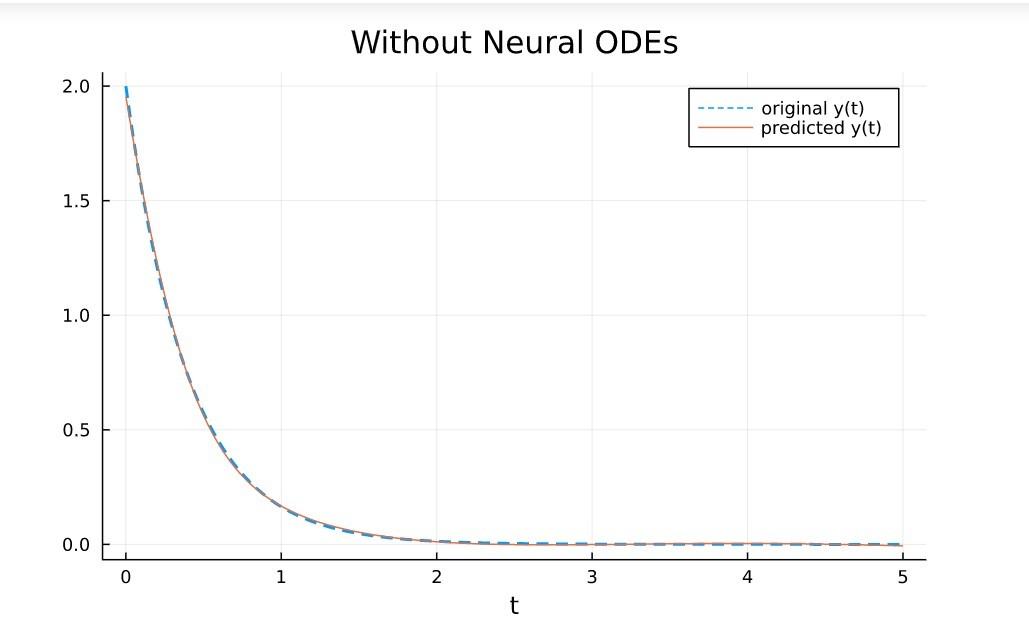
\includegraphics[width=6cm]{without ode.jpg}
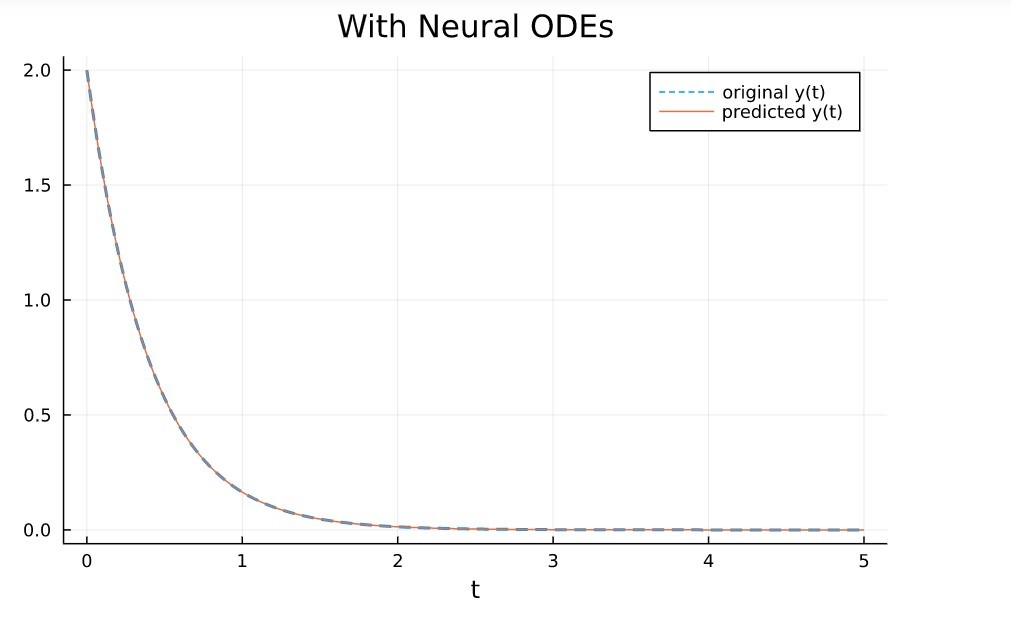
\includegraphics[width=6cm]{with ode.jpg}
    Figure 1: Visualization of the true value and approximation using neural networks with (left) and without ODE (right).
\end{center}

\begin{center}

\begin{tabular}{c|c|c|c}
    \hline
   MLP Model  & Time (s) & Memory Cost (M) & Loss \\
   \hline
   Without ODE	& 49.69	& 104.4	& $3.55*10^{-5}$ \\
    \hline
    With ODE & 165.6 &	323.6 &	$1.59*10^{-5}$ \\
    \hline
\end{tabular}

Table 1 Performance of neural network with and without ODE. Time (in second) and memory cost (in Mb) are measured by julia @time macro. Losses refer to mean-square error between training data and true value.
\end{center}


The figure and table above demonstrate the behavior of a multilayer perceptron (MLP) with and without ODE implementation. Both models had three layers containing 32 neurons per layer, and used ADAM for optimizer. In particular, Tsitouras 5/4 Runge-Kutta method (Tsit5) was used for solving the ODE problem on loss function $L(\mathbf{z})$, with default tolerance value $10^{-4}$. Under the same setting of time interval and training epochs = 500, MLP with ODE exhibited better accuracy than that without ODE, decreasing the loss by 56\%.

On the other hand, the training time and memory cost needed for MLP with ODE is about three times of that without ODE. This suggests that ODE-equipped neural networks may not be the best choice for training such simple exponential model. The large demand comes mainly from the backpropagation steps. But according to Chen et.al, training a neural ODE network requires constant memory cost if one does not store any intermediate values during the forward pass \cite{chen2019neural}. This means neural ODE could outweigh MLP for large daatsets in terms of memory cost.


\subsubsection{Training epochs and tolerance values}

\begin{center}
    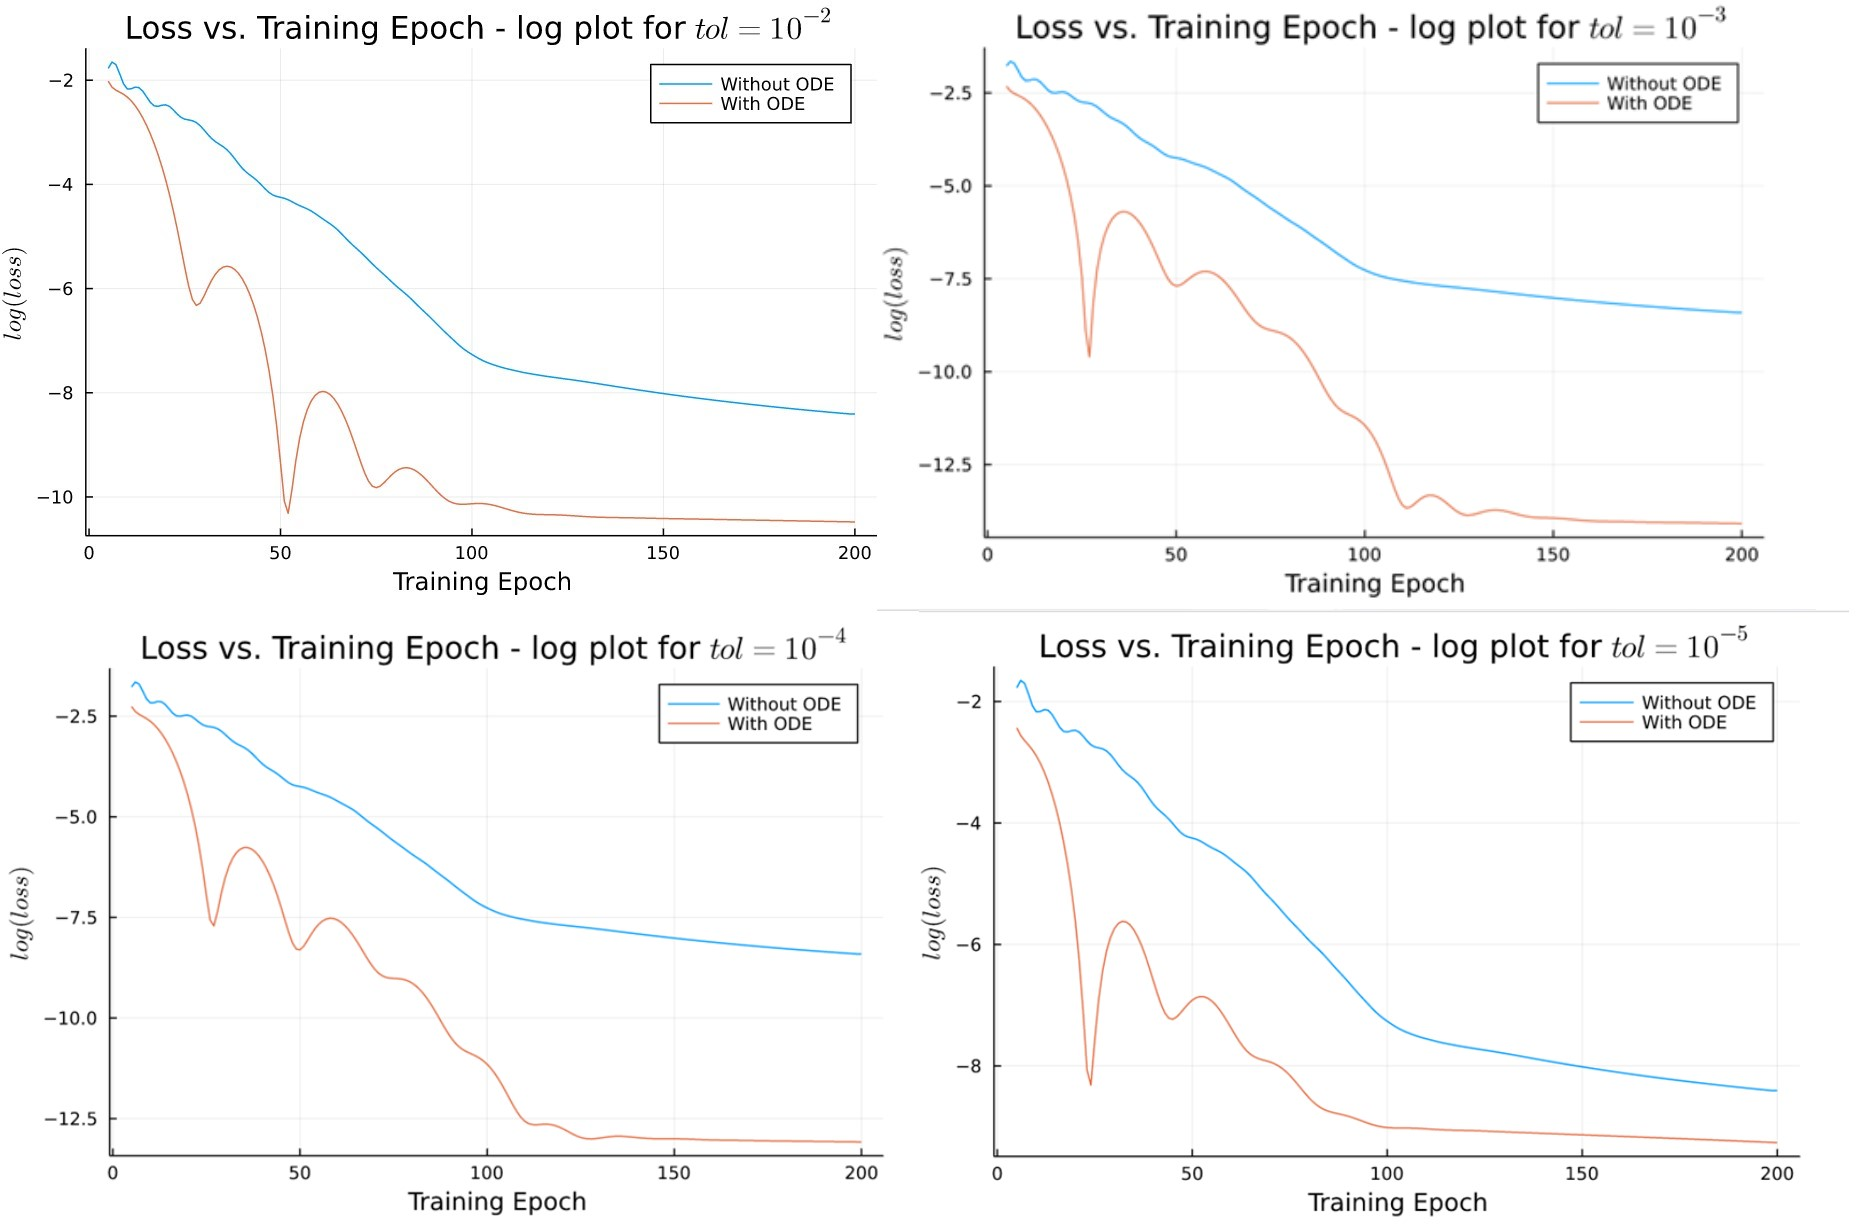
\includegraphics[width = 12cm]{tolerance values.jpg}
    Figure 2: Loss value for different tolerance settings
\end{center}
     
We tested the performance of neural ODE over different training epochs. According to the plots, both methods exhibit exponential relationships at first 100 epochs, and stabilize after epoch 100. But neural ODE shows better accuracy than normal neural network throughout the time, by a factor generally about $e^3 = 20$.

We further trained the model using different tolerance settings on the Tsit5 solver for the neural ODE network. Loss functions all tend to converge after 100 epochs. Therefore, epochs $=$ 100 is a reasonable setup for a neural ODE system. According to the plots, when epochs $>$ 100, two neural networks both converge much slower than prior steps. 

\begin{center}
    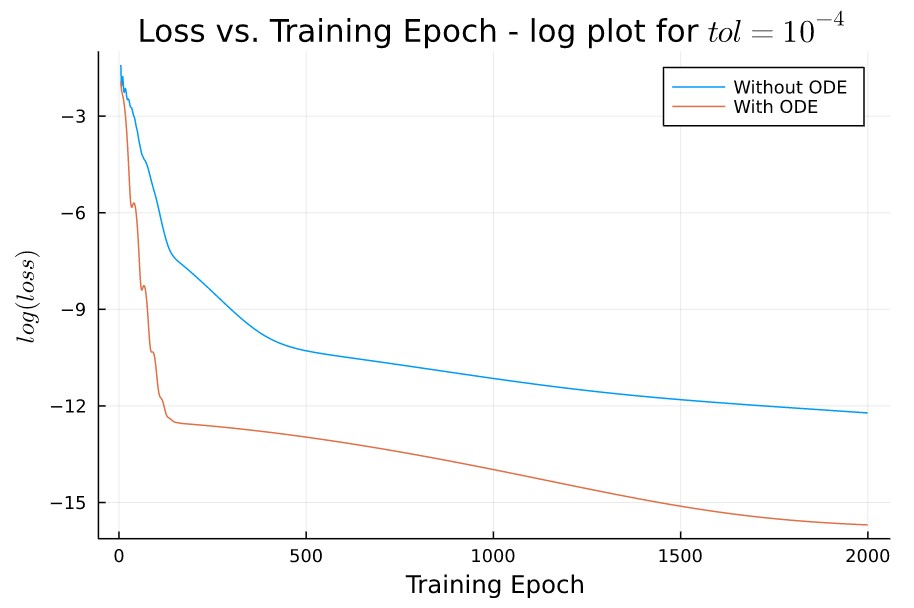
\includegraphics[width = 12cm]{2000 epochs.jpg}
    Figure 3: Loss value throughout training for 2000 epochs, tolerance = $10^{-4}$
\end{center}

In addition, we visualized the performance of two systems after training 2000 epochs. During later steps, although both systems converge much slower, neural ODE still has got a loss value lower than common neural network by a factor of $e^3 = 20$.

Surprisingly, the loss value does not decrease monotonically with tolerance settings. According to figure 2, for this specific neural ODE model, a $10^{-3}$ or $10^{-4}$ tolerance yields better accuracy than both $10^{-2}$ and $10^{-5}$. This is also reflected in the Neural ODE article. Chen et.al were able to reduce the tolerance to $10^{-3}$ and $10^{-5}$, respectively, without degrading performance compared to the default $1.5*10^{-8}$ setting \cite{chen2019neural}. 

Our study provides evidence and an even stronger result. There is one specific tolerance value most suitable for a given neural ODE system. Either increasing or decreasing the tolerance value would result in poorer accuracy. The reason why the relationship isn't monotonic actually comes from the complexity of the model itself - generally, lower, or stricter tolerance increases accuracy. However, this is under the assumption that we have infinitely more function evaluations and deeper model, which also leads to slower computations. In our training sample, we had a three-layer model, which naturally limits the accuracy when tolerance becomes too low. Thus, every data set has its own range of tolerance setting \cite{NeuralODEforecast}. Therefore, we suggest one may perform training on a toy data set to obtain this optimal tolerance value, before applying the neural ODE to solve real problems.

\subsection{Augmented NODE}

In certain cases, neural ODE might fail. According to a study by Dupont et.al, neural ODE cannot be applied to certain functions where the mapping trajectories intersect \cite{dupont2019augmented}. A simple example presented by them is the following function:  
$g_{1d}: \mathbb{R} \rightarrow \mathbb{R}$ be a function such that $g_{1d}(1) = -1, g_{1d}(-1) = 1$.
 
\begin{center}
    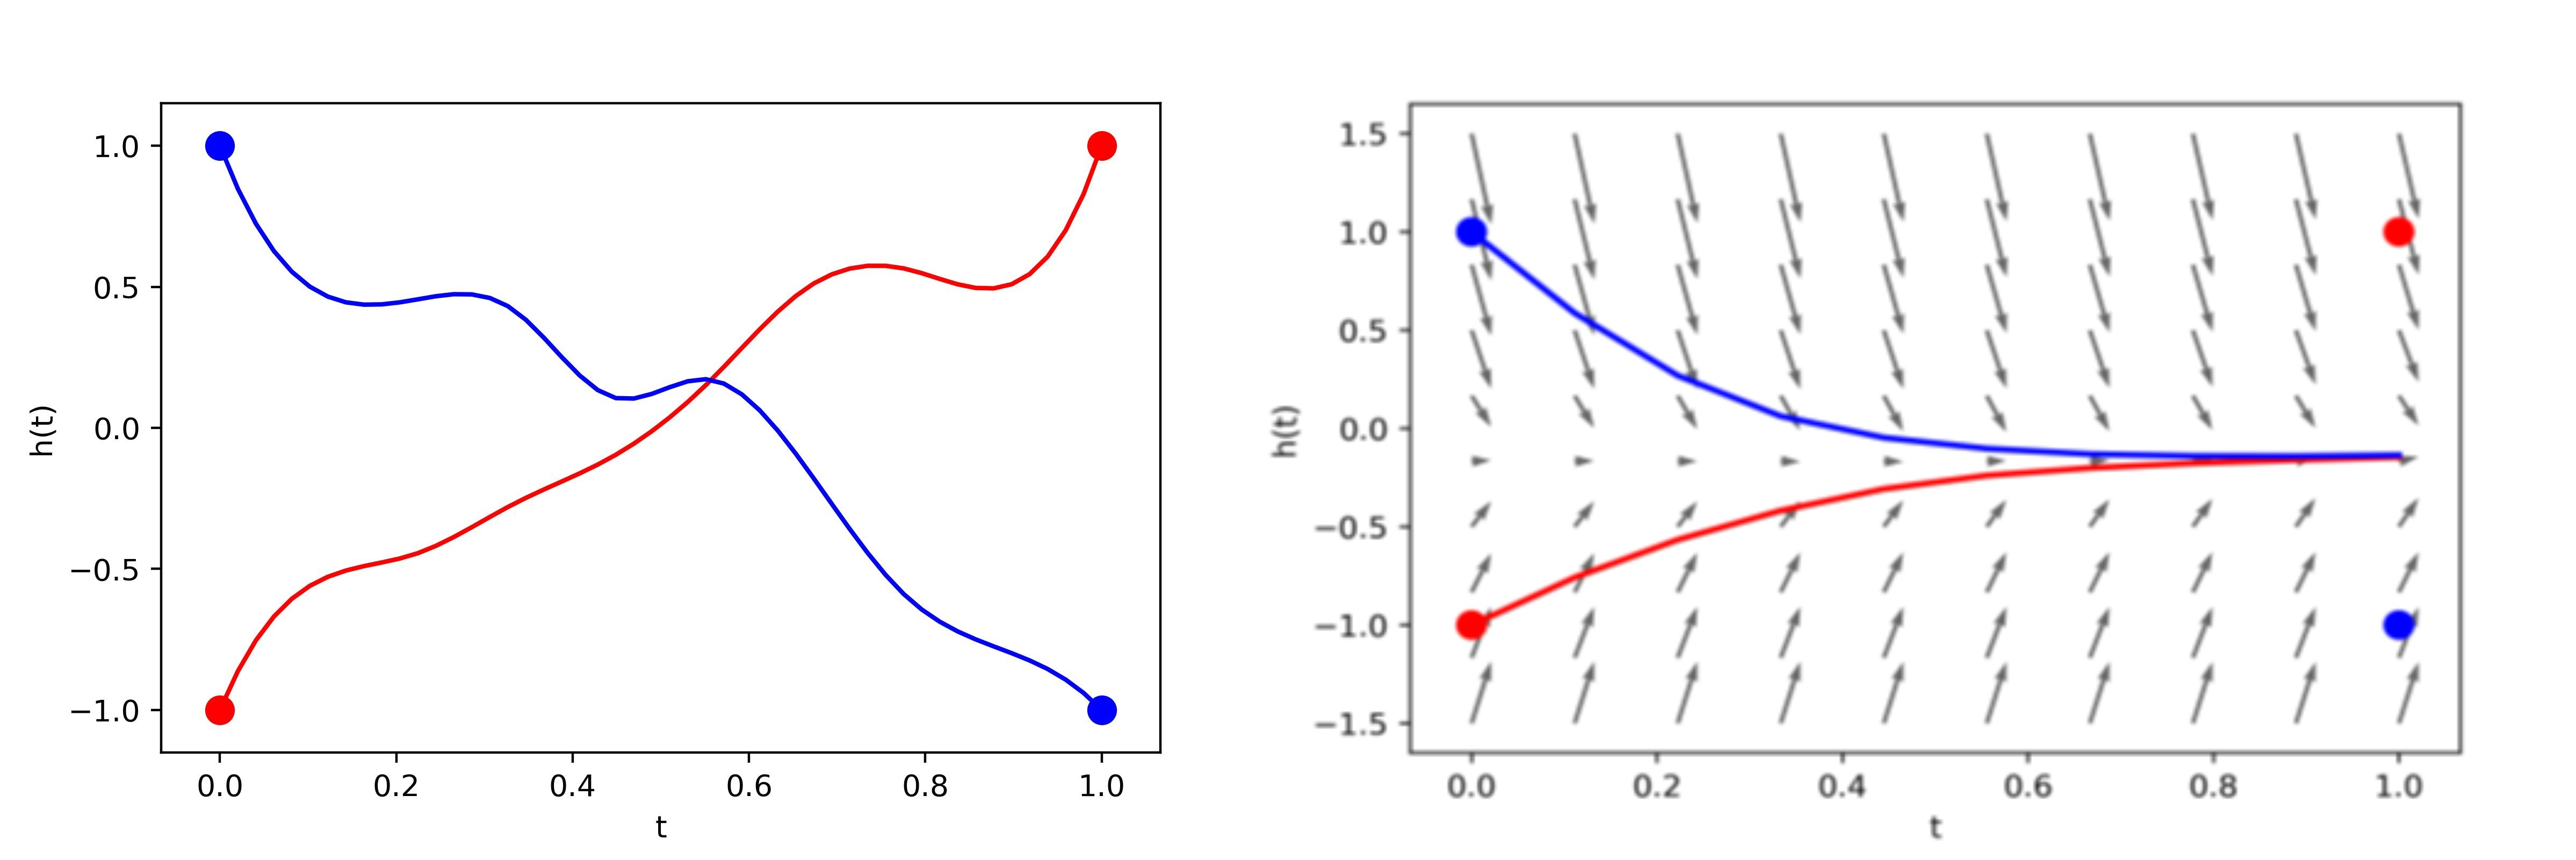
\includegraphics[width=12cm]{g1d.jpg}
    Figure 4 (Left) Continuous trajectories of the $g_{1d}$ mapping intersect with each other. (Right) Training an ODE fails to represent the $g_{1d}$ mapping \cite{dupont2019augmented}.
\end{center}

According to figure 4, the flow at every point can be easily learned using the gradient, and the flow can be easily generated. It’s impossible to represent this function using an ODE. Since the solution starting from any point in the space is uniquely determined by the vector field, two ODE trajectories can never intersect. However, the trajectories of $g_{1d}(-1)$ and $g_{1d}(1)$ must intersect according to intermediate value theorem. This leads to failure of training the system using neural ODE. This deviation is shown in figure 5.

To overcome this difficulty, Dupont et.al introduced augmented neural ODEs (ANODEs) \cite{dupont2019augmented}. They augment the space for learning from $\mathbb{R}_n$to $\mathbb{R}_{n+p}$. In other words, they concatenate every data point with a vector of zeros $\mathbf{a}(t)\in \mathbb{R}_p$. Then the ODE can be formulated as:  
$\frac{d}{dt}
\begin{bmatrix}
\mathbf{z}(t) \\
\mathbf{a}(t)
\end{bmatrix} = f(\begin{bmatrix}
\mathbf{z}(t) \\
\mathbf{a}(t)
\end{bmatrix} , t), \begin{bmatrix}
\mathbf{z}(0) \\
\mathbf{a}(0)
\end{bmatrix} = \begin{bmatrix}
\mathbf{x} \\
\mathbf{0}
\end{bmatrix}
$, where $\mathbf{x}$ is a input data point.

The reason behind this is that adding the extra zero vector increases the dimension of $\mathbf{z}(t)$. In this way, the trajectories would not intersect in higher dimensions. They also hypothesized that this will also make the augmented $f$ smoother, giving rise to simpler flows that the ODE solver can compute in fewer steps.

\begin{center}
    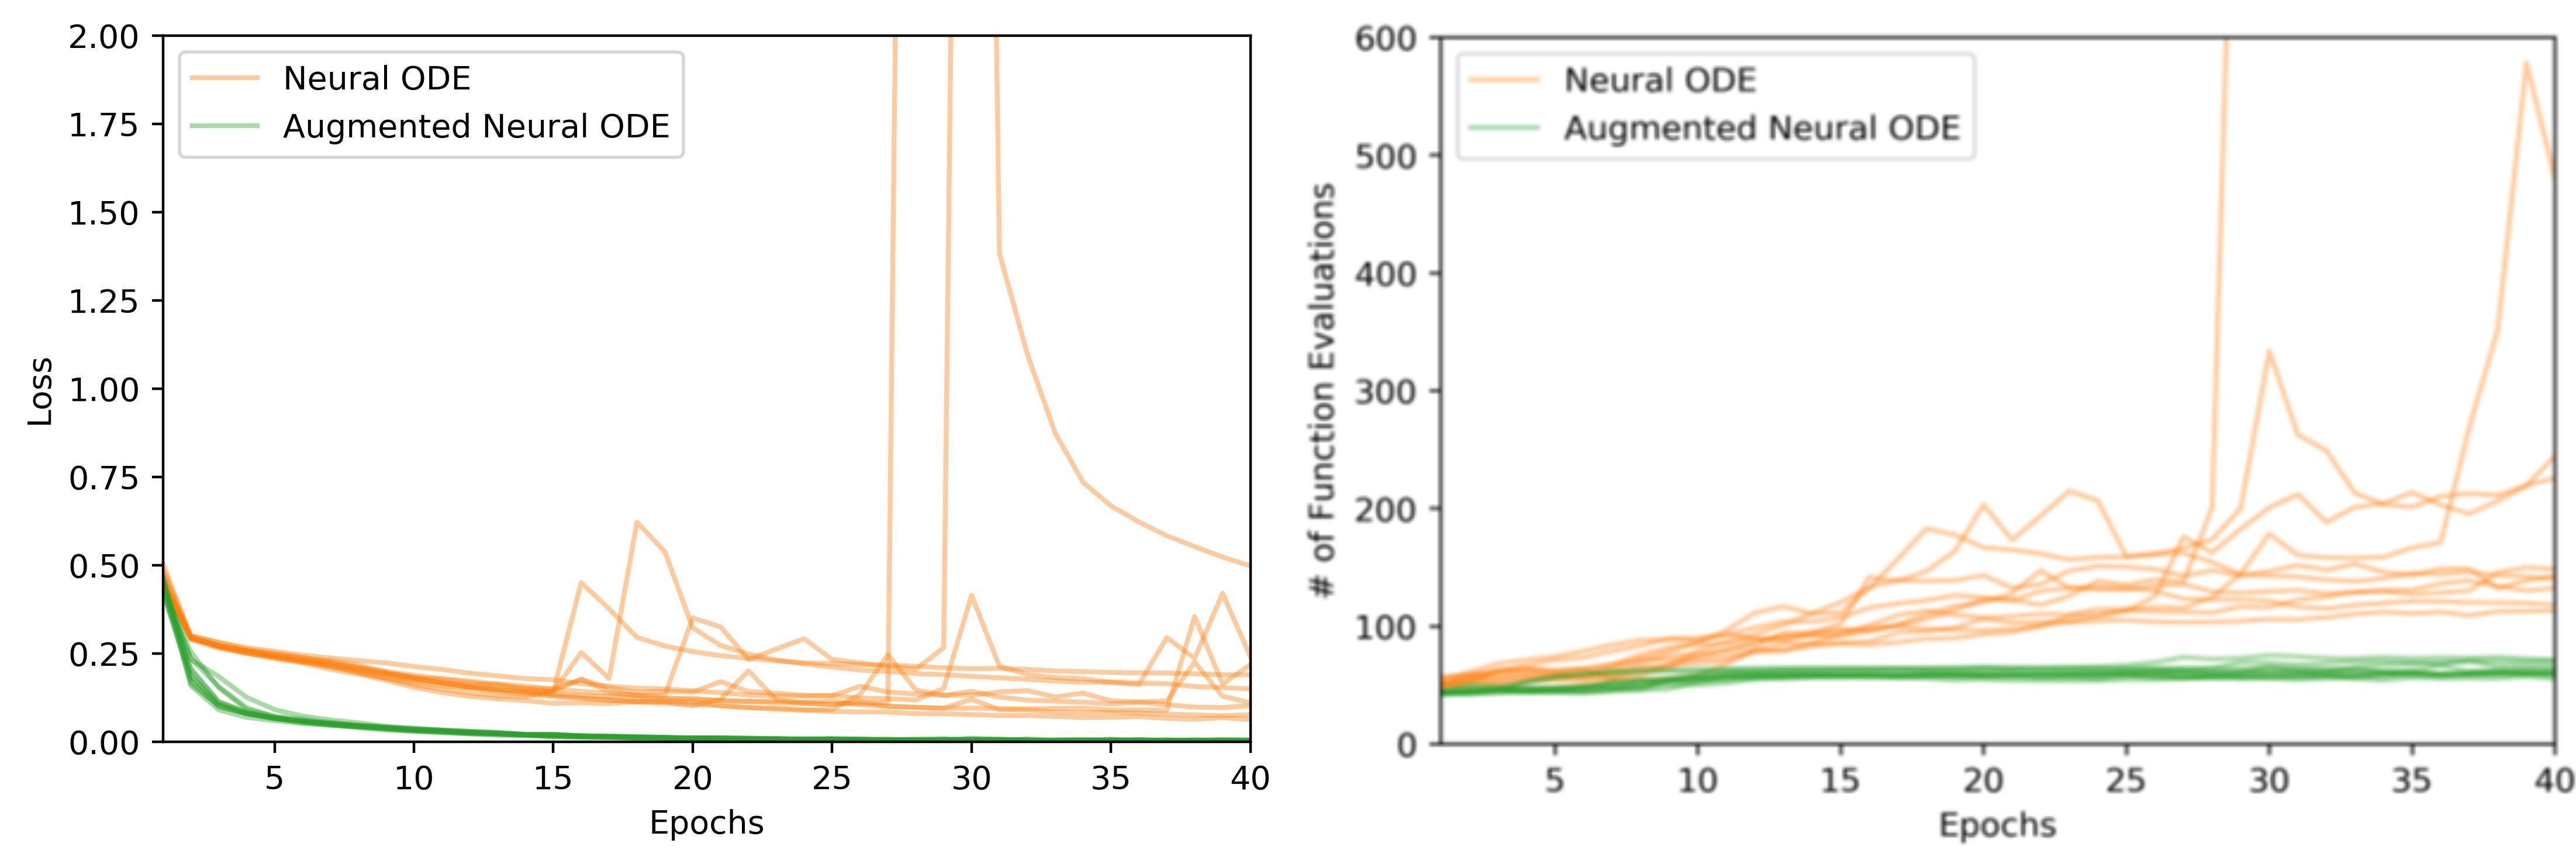
\includegraphics[width = 12cm]{instability.jpg}
    Figure 5: Instability in terms of loss (left) and NFE (right) in the latter stage of training NODE
\end{center}   

Figure 5 shows the loss and number of function evaluations (NFE) throughout training periods. The trainings were carried out by Dupont et.al over the NMIST dataset. \cite{NMIST} NODE is unstable in later training periods. But on the other hand, ANODE remains stable throughout the training period. Besides, the loss of ANODE is also constantly less than that of NODE \cite{dupont2019augmented}. The figure suggests that augmented neural ODE is not only able to solve problems that cannot be achieved by training neural ODEs, but also performs better in terms of training loss and stability. Therefore, augmented neural ODE could be a better choice when solving character recognition problems.

\section{Conclusion}
In this study, we inspected the loss and memory cost of algorithms with and without ODEs. Through visualization, we noticed that in specific examples, the losses are similar for both methods, but computing without ODEs takes up only around a third of the memory. One improvement of neural ODE is augmented neural ODE, which can be applied in more cases and remain stable over more test periods.

\section{Author contribution}
XR and LT conceived of the current idea. LT designed and implemented the neural ODE model, and performed loss and analysis visualizations. LT and XR wrote the manuscript: LT contributed to section 1.4, 2.1, and 2.2; XR contributed to abstract $\&$ section 1.1, 1.2, 1.3, 1.4, and 3. LT performed   $LaTeX$ formatting.

\printbibliography

\end{document}
